¿Cuál es el \'area del trapecio de la figura \ref{fig:area_compuesta_03}?

\begin{figure}[H]
    \begin{center}
        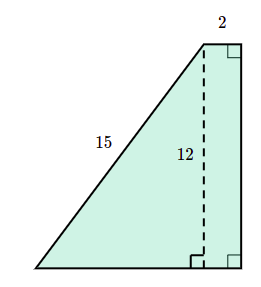
\includegraphics[width=0.2\linewidth]{../images/area_compuesta_03.png}
    \end{center}
    \caption{}
    \label{fig:area_compuesta_03}
\end{figure}
\begin{solutionbox}{15cm}

    \begin{minipage}{0.7\textwidth}
        Para determinar el área del trapecio debemos saber la longitud del cateto del triángulo rectángulo. Llamemos $x$ a la longitud (ver Figura \ref{fig:area_compuesta_03a}).
        Cuando tenemos un triángulo rectángulo, podemos usar el teorema de Pitágoras para obtener la longitud del cateto.
        La ecuación para el teorema de Pitágoras es:
        \[c^2=a^2+b^2\]
        En este caso, $a=12$, $b=x$ y $c=15$, Entonces,
        \begin{align*}
            12^2+x^2 & =15^2    \\
            144+x^2  & =225     \\
            x^2      & =225-144 \\
            x^2      & =81      \\
            x        & =9
        \end{align*}
        La longitud del cateto es 9. Ahora vamos a usar la altura para determinar el área de ambas partes del trapecio.
        Primero, el rectángulo (ver Figura \ref{fig:area_compuesta_03b}):
        \begin{align*}
            A & =bh        \\
            A & =2\cdot 12 \\
            A & =24
        \end{align*}
        Ahora vamos a determinar el área de la porción triangular del trapecio (ver Figura \ref{fig:area_compuesta_03c}):
        \begin{align*}
            A & =\frac{1}{2}bh        \\
            A & =\frac{1}{2}9\cdot 12 \\
            A & =54
        \end{align*}
        Podemos sumar las áreas de las dos partes para determinar el área total del trapecio.
        \[24+54=78 \text{ u}^2\]
    \end{minipage}\hfill
    \begin{minipage}{0.25\textwidth}
        \begin{figure}[H]
            \centering
            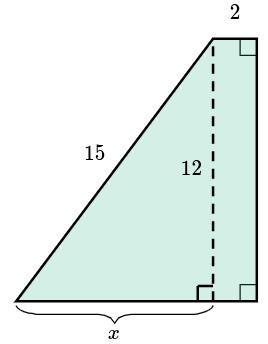
\includegraphics[width=0.5\linewidth]{../images/area_compuesta_03a.png}
            \caption{}
            \label{fig:area_compuesta_03a}
        \end{figure}
        \begin{figure}[H]
            \centering
            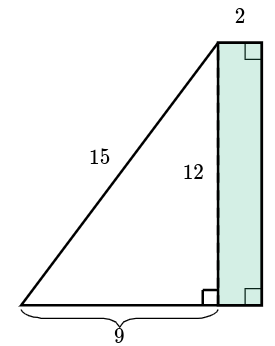
\includegraphics[width=0.5\linewidth]{../images/area_compuesta_03b.png}
            \caption{}
            \label{fig:area_compuesta_03b}
        \end{figure}
        \begin{figure}[H]
            \centering
            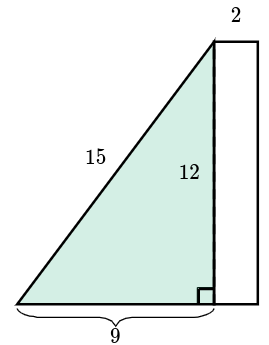
\includegraphics[width=0.5\linewidth]{../images/area_compuesta_03c.png}
            \caption{}
            \label{fig:area_compuesta_03c}
        \end{figure}
    \end{minipage}

\end{solutionbox}